%%%%%%%%%%%%%%%%%%%%%%%%%%%%%%%%%%%%%%%%%%%%%%%%%%%%%%%%%%%%%%%%%%%%%%%%%%%%%%%%%%
\begin{frame}[fragile]\frametitle{}
\begin{center}
{\Large TensorFlow Quantum}
\end{center}
\end{frame}

%%%%%%%%%%%%%%%%%%%%%%%%%%%%%%%%%%%%%%%%%%%%%%%%%%%%%%%%%%%
 \begin{frame}[fragile]\frametitle{Introduction}
 
\begin{itemize}
\item  While a normal Turing machine can only perform one calculation at a time, a quantum Turing machine can perform many calculations at once.
\item  TFQ adds the ability to process quantum data, consisting of both quantum circuits and quantum operators. 
\end{itemize}

\begin{center}
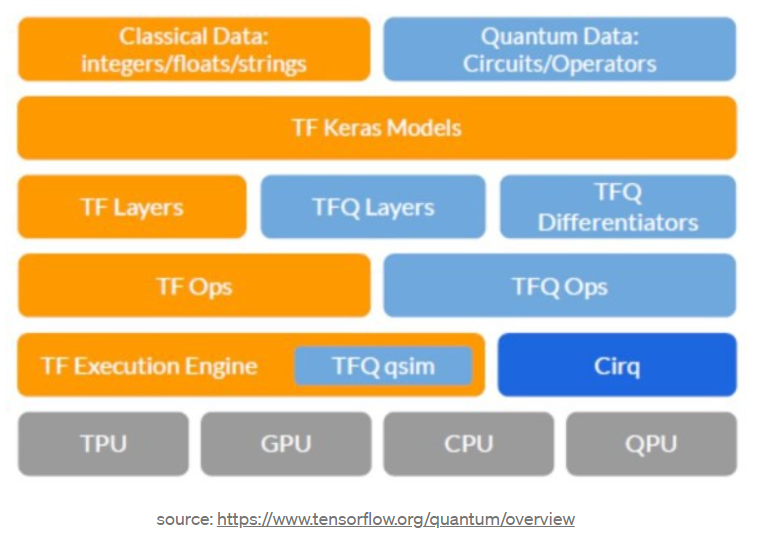
\includegraphics[width=0.6\linewidth,keepaspectratio]{tfq}
\end{center}
	
	
\tiny{(Ref: TensorFlow Quantum: beauty and the beast  - Shubham Goyal)}

\end{frame}

%%%%%%%%%%%%%%%%%%%%%%%%%%%%%%%%%%%%%%%%%%%%%%%%%%%%%%%%%%%
 \begin{frame}[fragile]\frametitle{TFQ Steps}
 
 TFQ steps to train and build QML models:
 
\begin{itemize}
\item  Prepare a quantum dataset: Quantum data is loaded as tensors, specified as a quantum circuit written in Cirq. The tensor is executed by TensorFlow on the quantum computer to generate a quantum dataset.
\item  Evaluate a quantum neural network model: prototype a quantum neural network using Cirq that will be embedded inside of a TensorFlow compute graph.
\item  Sample or Average: This step leverages methods for averaging over several runs involving steps (1) and (2).
\item  Evaluate a classical neural networks model: This step uses classical deep neural networks to distill such correlations between the measures extracted in the previous steps.
\item  Evaluate Cost Function: Similar to traditional machine learning models, TFQ uses this step to evaluate a cost function.
\item  Evaluate Gradients \& Update Parameters.
\end{itemize}

	
\tiny{(Ref: TensorFlow Quantum: beauty and the beast  - Shubham Goyal)}

\end{frame}

%%%%%%%%%%%%%%%%%%%%%%%%%%%%%%%%%%%%%%%%%%%%%%%%%%%%%%%%%%%
 \begin{frame}[fragile]\frametitle{QML Learning}
 

\begin{itemize}
\item  In quantum neural networks we’ll be feeding our input data embedded into quantum bits, aka qubits, and so any operations applied onto that form will need to be conducted by aggregations of quantum gates applied sequentially to and between those qubits through the progression of time steps. With each of these gate operations, we’ll be rotating the superposition state around an axis of those qubits’ “Bloch spheres”.
\item Quantum algorithms are means to craft by such gate rotations a shaped superposition of collective qubit states such that the probabilistic measurement operations on the returned qubit states are more likely to collapse to classical states corresponding to some desired output.
\item  Each layer of gates only interacts with adjacent qubits instead of all to all. This reduced information flow is compensated by the depth of information capacity of multi-qubit superpositions.

\end{itemize}

	
\tiny{(Ref: QML Learning with TensorFlow Quantum - Nicholas Teague)}

\end{frame}

%%%%%%%%%%%%%%%%%%%%%%%%%%%%%%%%%%%%%%%%%%%%%%%%%%%%%%%%%%%
 \begin{frame}[fragile]\frametitle{QML Learning}
 

\begin{itemize}
\item The realized gated network can then be given a form of supervised training to fit the parameterized gate sets to result in a returned superposition more aligned with our target state as a function of inputs. 
\item  The chain rule of backpropagation doesn’t directly translate to quantum primitives. However, there is a very clean solution realized by the simple modularity inherent in the networks. In other words, if in a forward pass the returned measurements from a quantum network are fed as input to a classical network, then in the backward pass we can simply apply the returned gradients from the classical network as input to the gradient calculations of the quantum network.
\end{itemize}

	
\tiny{(Ref: QML Learning with TensorFlow Quantum - Nicholas Teague)}

\end{frame}